\section{Battery Meter}
Using an Arduino, I made a circuit to display the approximate capacity left in a VEX battery.

\begin{figure}[h]
    \centering
    \includegraphics[width=\textwidth,height=5cm,keepaspectratio=true]{BatteryTester/circuit}
    \includegraphics[width=\textwidth,height=5cm,keepaspectratio=true]{BatteryTester/BatteryTesterSetup}
    \caption{
        (Left) The circuit. (Right) The circuit on a breadboard.
    }
\end{figure}

At the most basic level, the circuit works by using a voltage divider to measure the voltage of any battery up to 12v; All the other wires are to power the LCD and arduino. After that, I used math to display the approximate battery life left as a function of voltage.

This how other devices measure battery life however. Your phone, for example, actively measures every bit of charge that comes in and out of your phone and uses calculus to give a accurate battery percent \cite{CoulombCounting}. Simpler devices instead integrate voltage over time on a known dischage curve \cite{IntegrationVoltage} and use that to give a slightly less accurate estimation of battery. I didn't use either since I don't know calculus yet.

\begin{figure}[h]
    \centering
    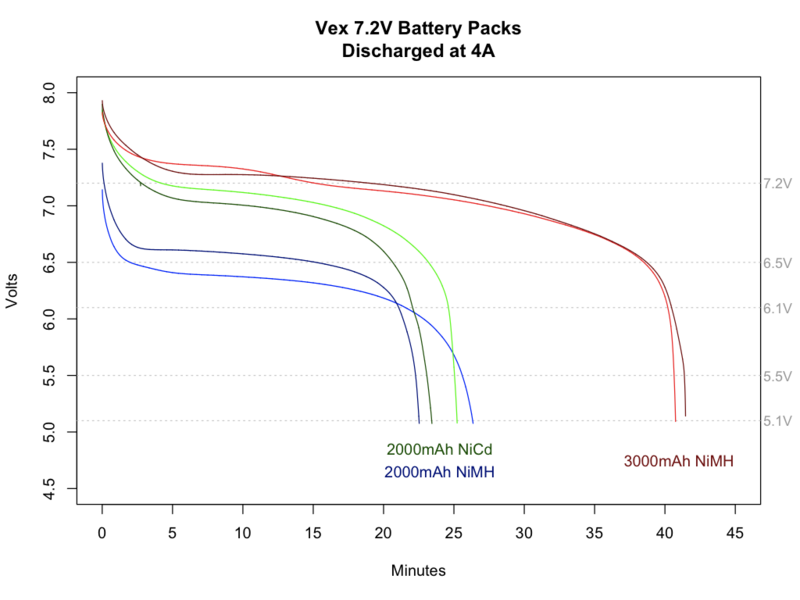
\includegraphics[width=\textwidth,height=7cm,keepaspectratio=true]{BatteryTester/DischargeGraph}
    \caption{
        The VEX battery's discharge curve over various currents, thanks to Quazar \cite{Quazar}. Notice how the voltage virtually levels out during the majority of its lifetime; This makes it difficult to get an approximate percent throughout the entire lifetime of the battery with just voltage without using integration.
    }
\end{figure}

To try to at least an accurate reading without calculus, I made a discharge curve using 2 motors as the load over time and made it a function of voltage (This was inspired by how Renegade Robotics \cite{RenegadeRobotics} does it). With this function, I was able to determine the approximate remaining battery capacity of our battery by measuring it's unloaded voltage.

\begin{figure}[h]
    \centering
    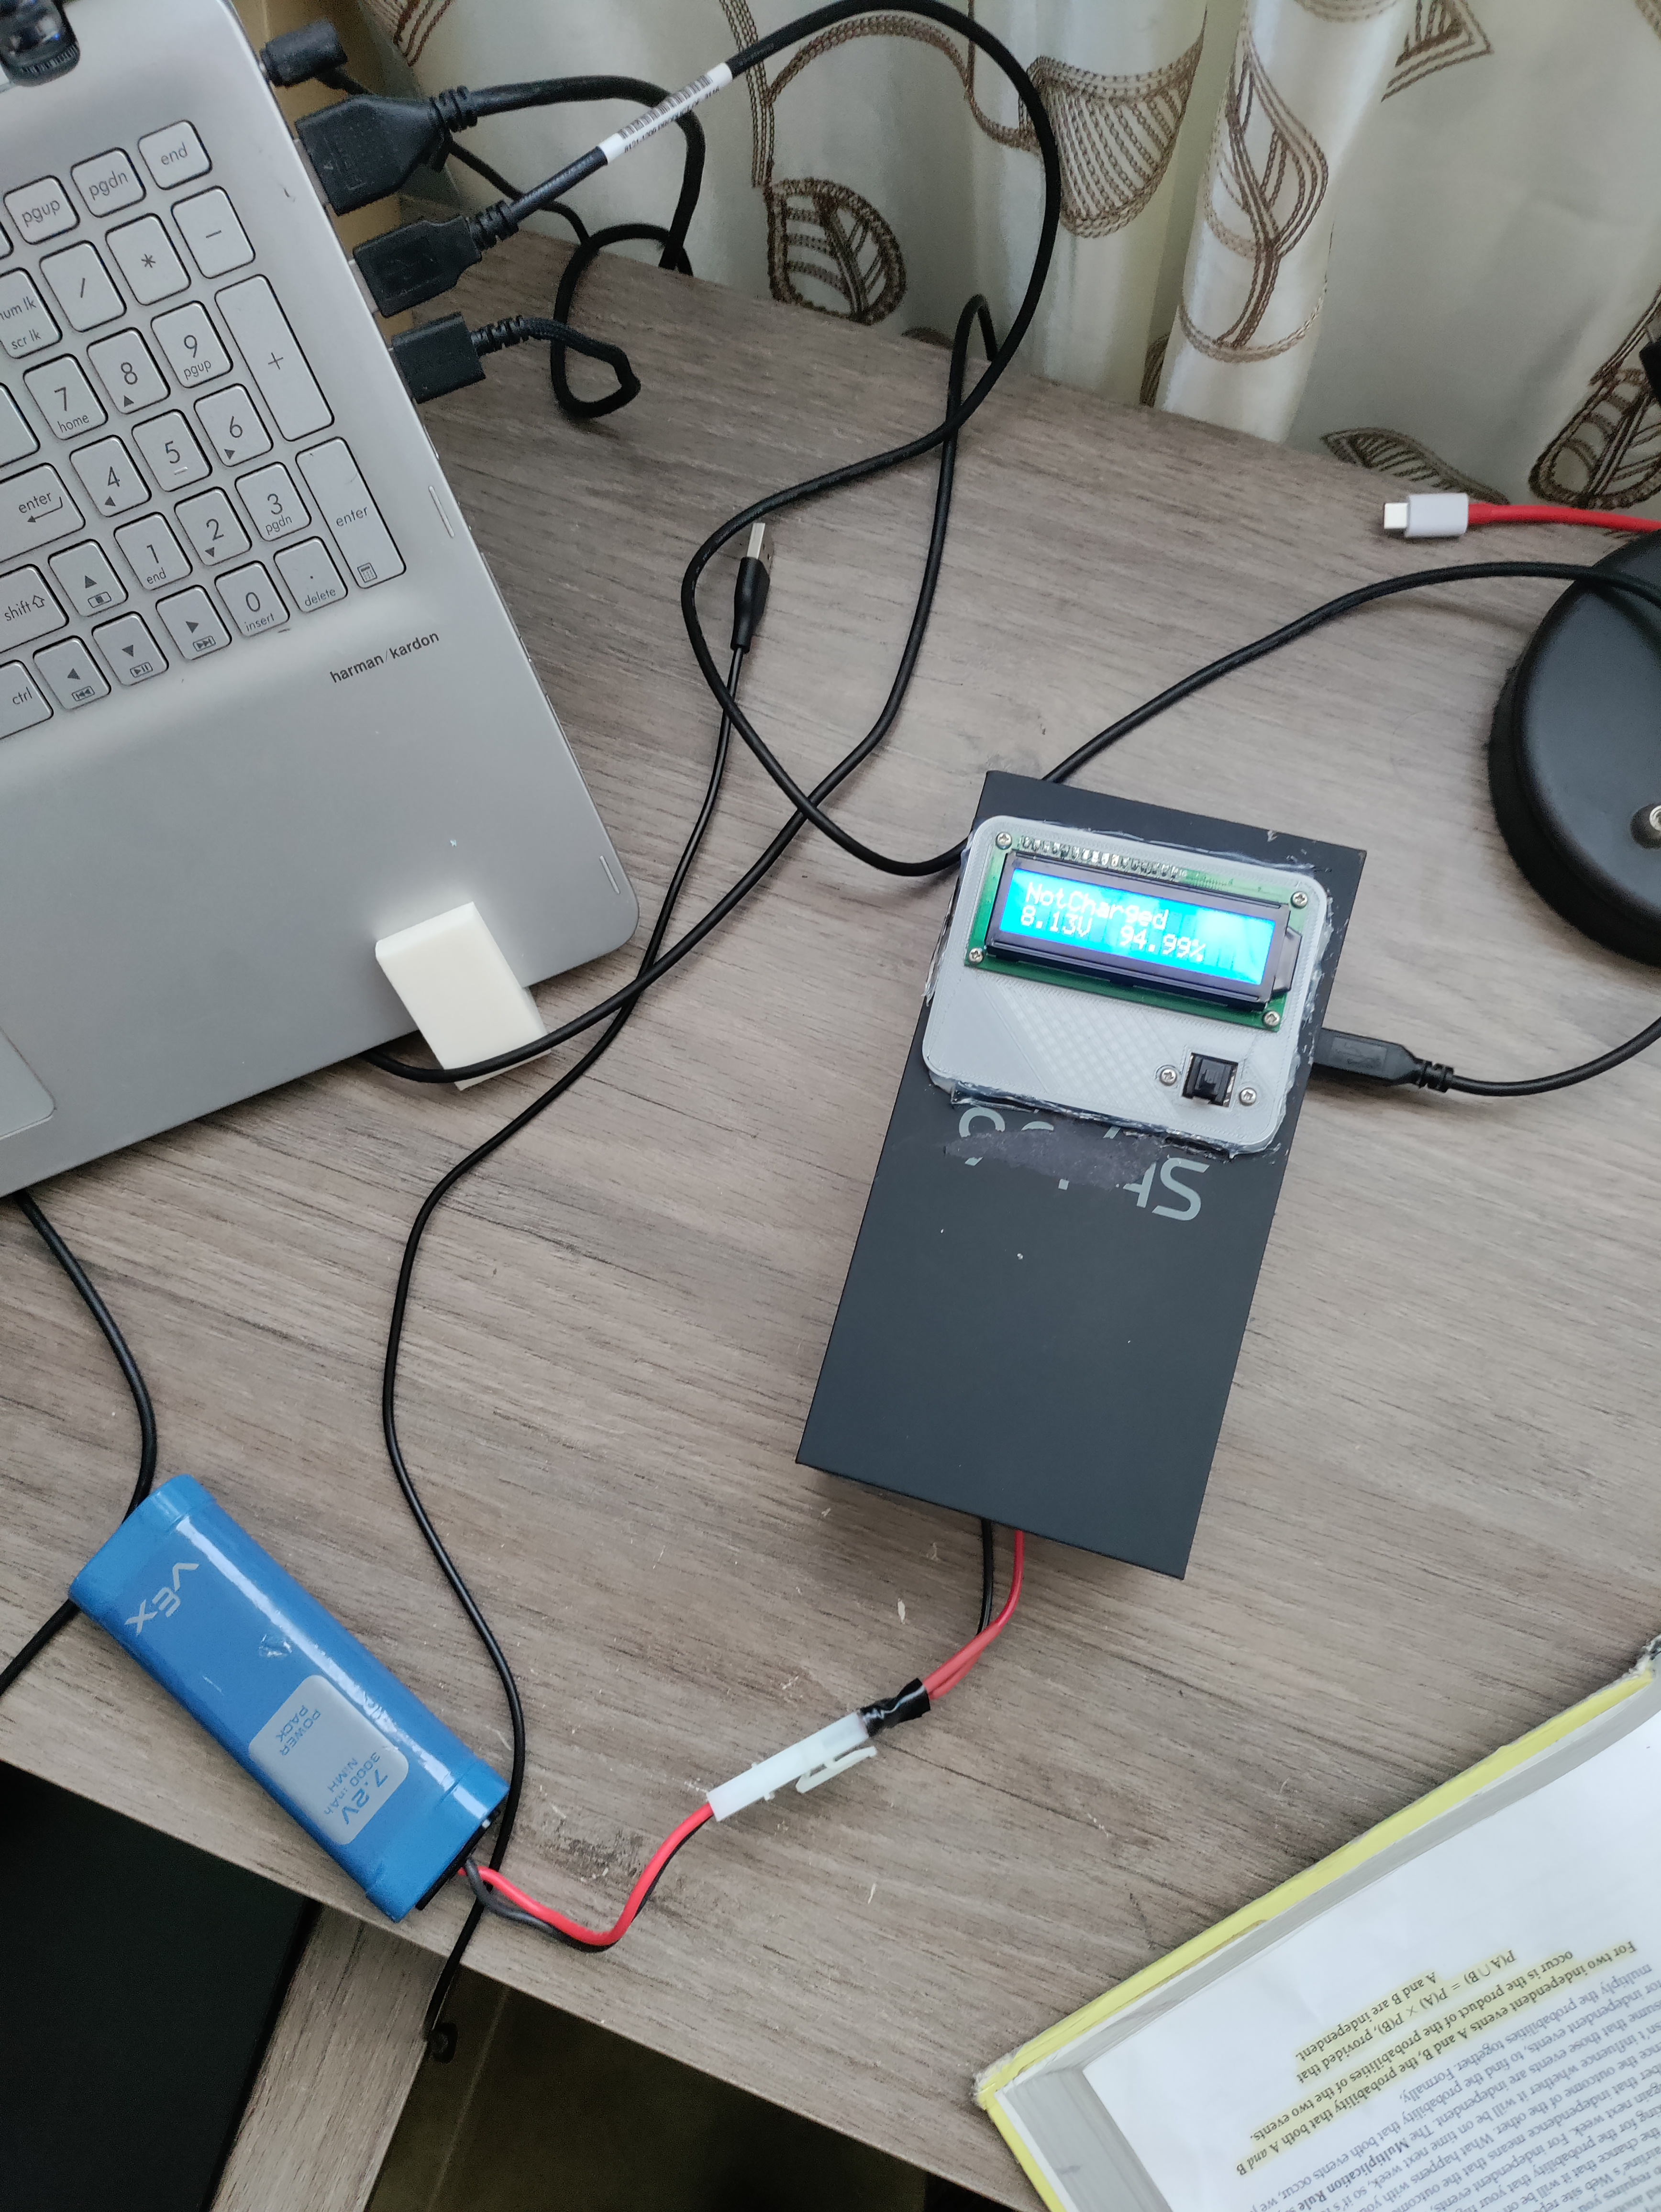
\includegraphics[width=\textwidth,height=7cm,keepaspectratio=true]{BatteryTester/BatteryTesterPortable}
    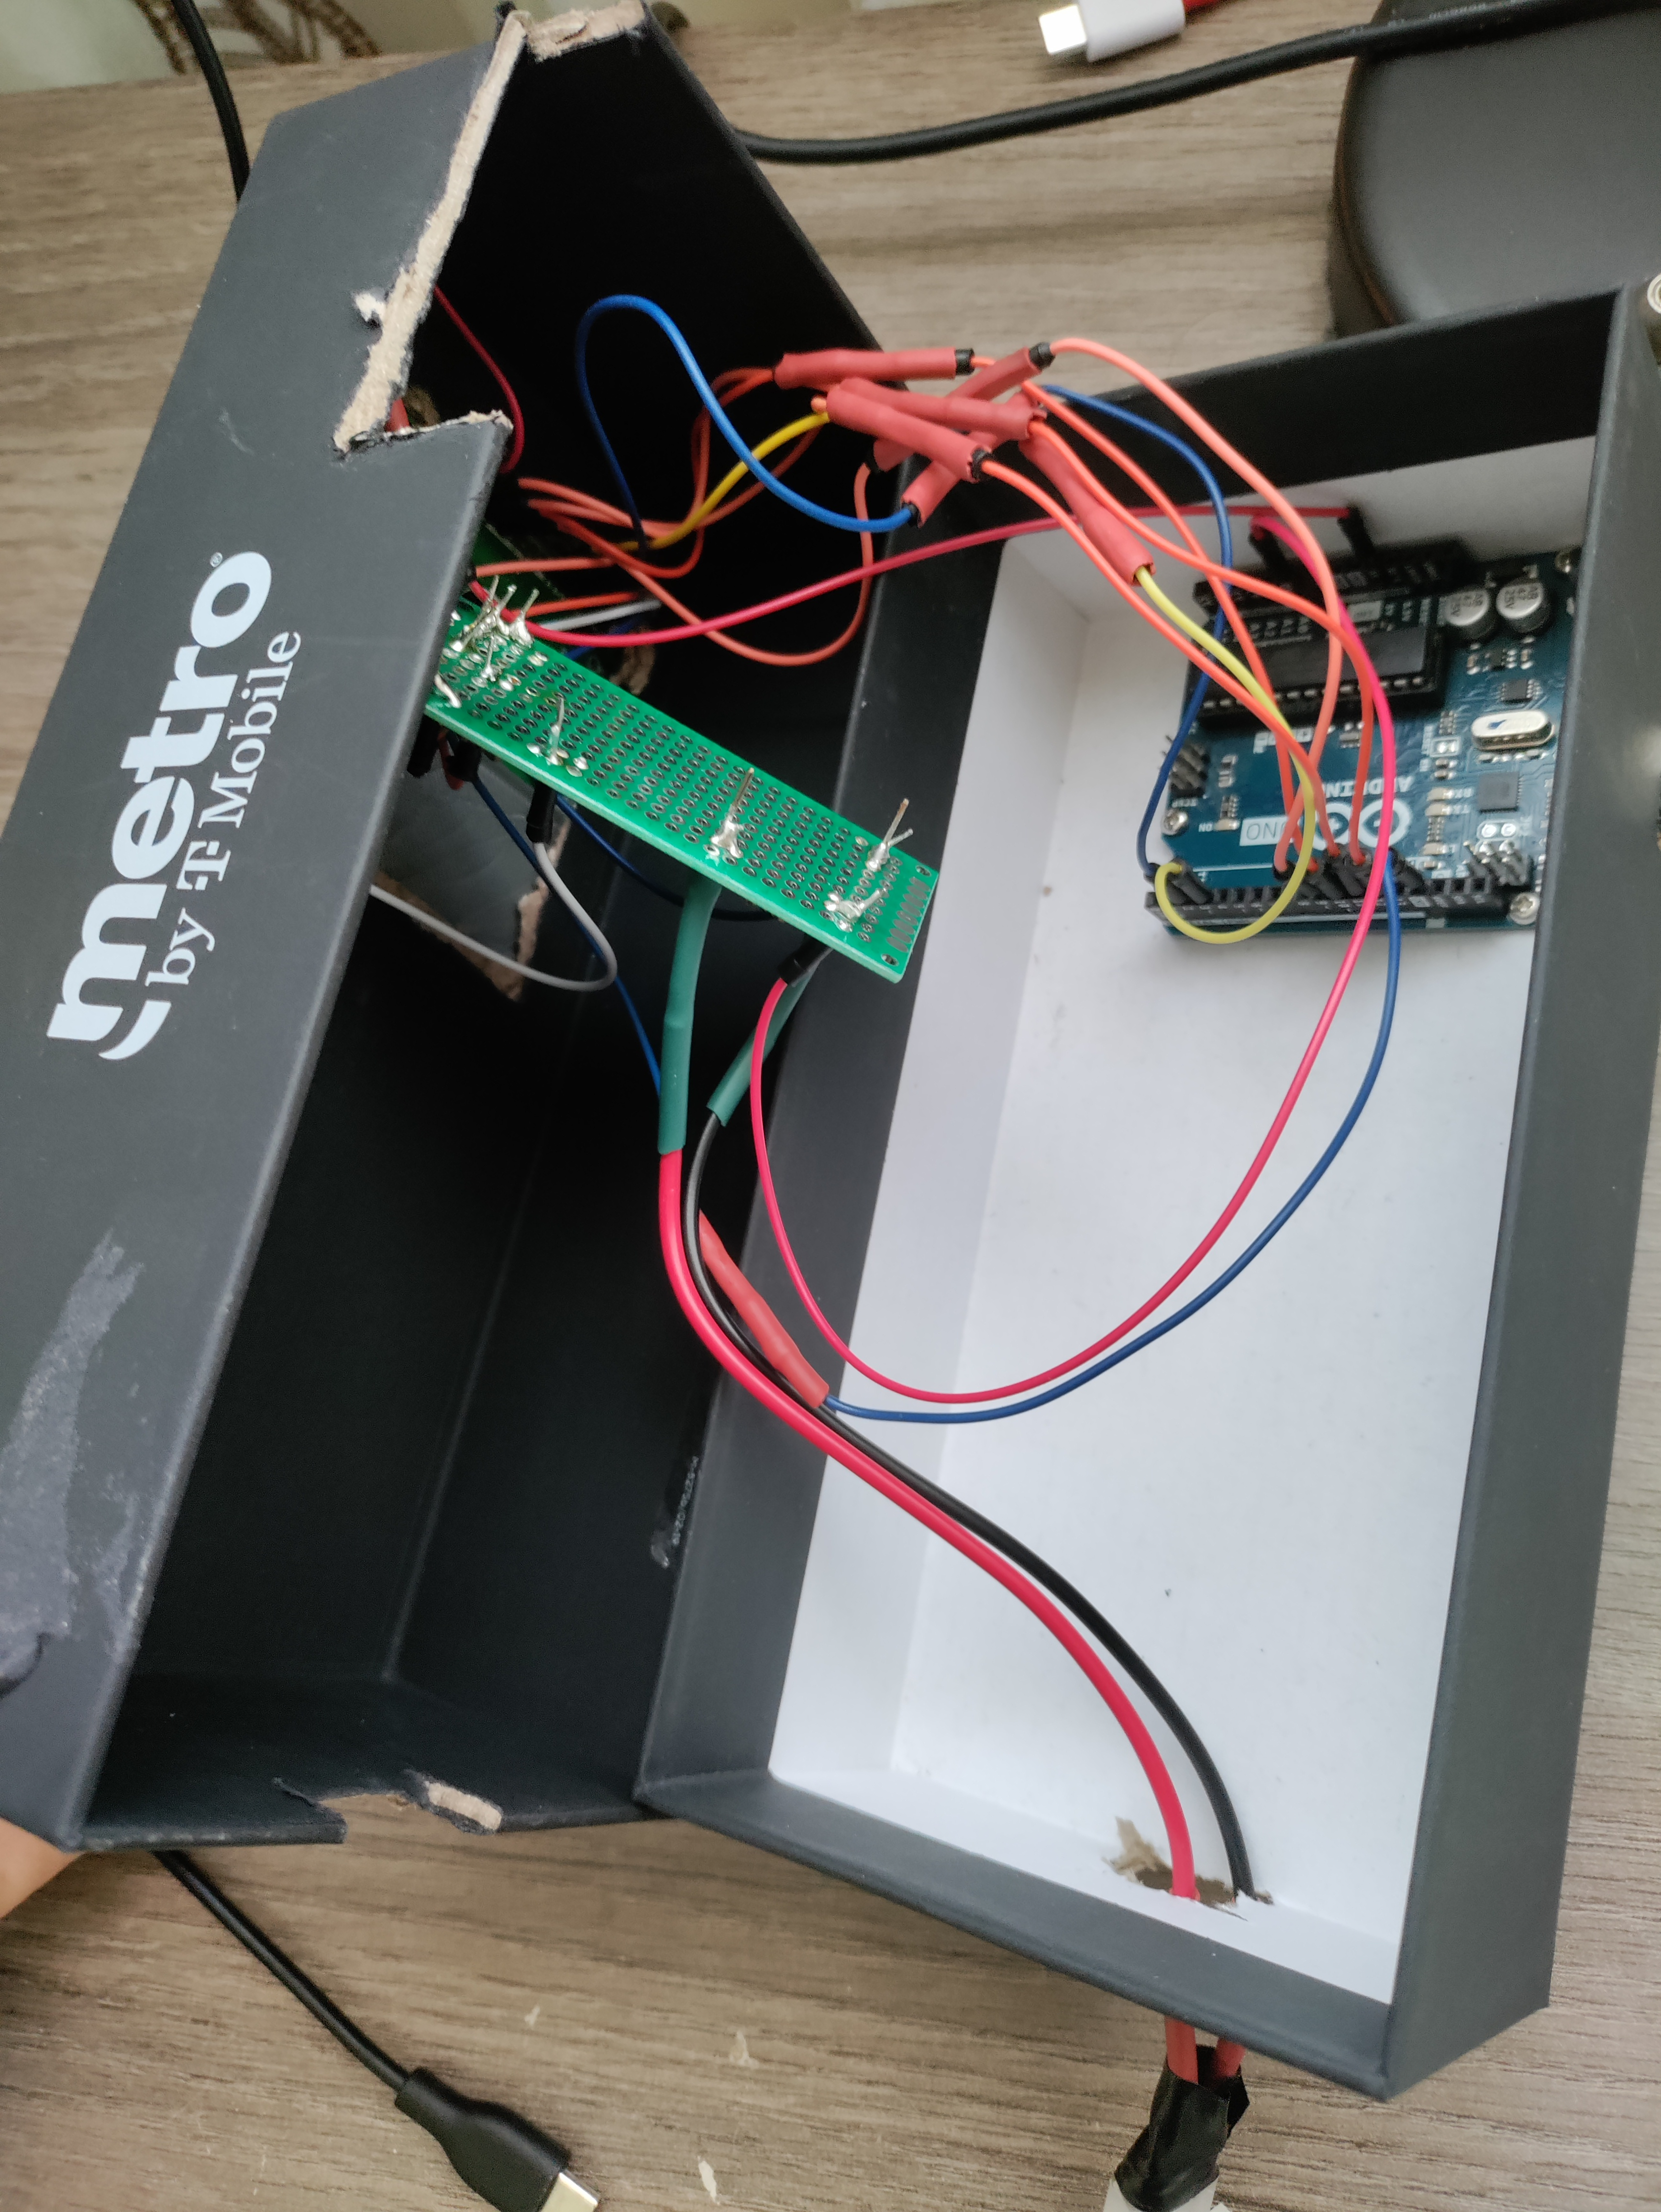
\includegraphics[width=\textwidth,height=7cm,keepaspectratio=true]{BatteryTester/BatteryTesterPortInside}
    \caption{
    The portable version of this project crammed into an old phone box. A blank PCB was used instead of a breadboard in this version to prevent the battery from accidentally shorting itself in the case it were ever dropped. The button is used to toggle the backlight to control power consumption, so that it can be powered by a mobile battery efficiently.
    }
\end{figure}

After that, I crammed the electronics into an old phone box, used leftover screws and nuts to secure its components, and called it a day.
